\documentclass[oneside,a4paper,12pt]{article}
\usepackage{graphicx}
\usepackage{amsmath}
\usepackage{listings}
\usepackage{array}
\usepackage{subcaption}
\usepackage{caption}
\usepackage{biblatex}
\addbibresource{rapport.bib}
\usepackage{hyperref}
\graphicspath{{~/templates/}, {../images/}}

\makeindex
\begin{document}
	\begin{titlepage}
		\includegraphics[width=4cm]{logopopo.png}
		\hspace*{\fill}
		\includegraphics[width=6cm]{logouniv.png}
		
		\begin{center}
			\vspace{1cm}
			\textbf{Mémoire de Stage de 4e année}\\
			\vspace{1cm}
			\textbf{\LARGE FL-Minifer}\\
			\textbf{\large A Tool To Minify and Unify AdBlocker’s Filter Lists}\\
			\vspace{1cm}
			\textbf{Maxence NEUS}\\
			\vspace{1cm}
			\begin{tabular}{ c c }
				
\includegraphics[width=6cm]{logoInria.jpg} & 
\includegraphics[width=6cm]{logospirals.png}\\
			\end{tabular}

			\vspace{2cm}

			\begin{tabular}{ m{6cm} | m{6cm} }
				\textbf{Polytech Lille} & \textbf{Inria} \\
				\hline
				& \\
				Secrétariat - Bureau & 40 Av. Halley \\
				Boulevard Paul Langevin - Cité Scientifique & 59650 Villeneuve d'Ascq \\
				59655 VILLENEUVE D’ASCQ CEDEX & Tuteur Entreprise : \\
				03-28-76-73-60 & \textbf{Walter RUDAMETKIN} \\
				03-28-76-73-61 & Tuteur Ecole \\
				\includegraphics[width=2.5cm]{logouniv.png} \includegraphics[width=2.5cm]{logopopo.png} & \textbf{Walter RUDAMETKIN} \\
				
			\end{tabular}
			
			\vspace{\fill}
			\textbf{2022}\\
		\end{center}
	\end{titlepage}

\tableofcontents

\newpage

\begin{figure}[h]
	\centering
	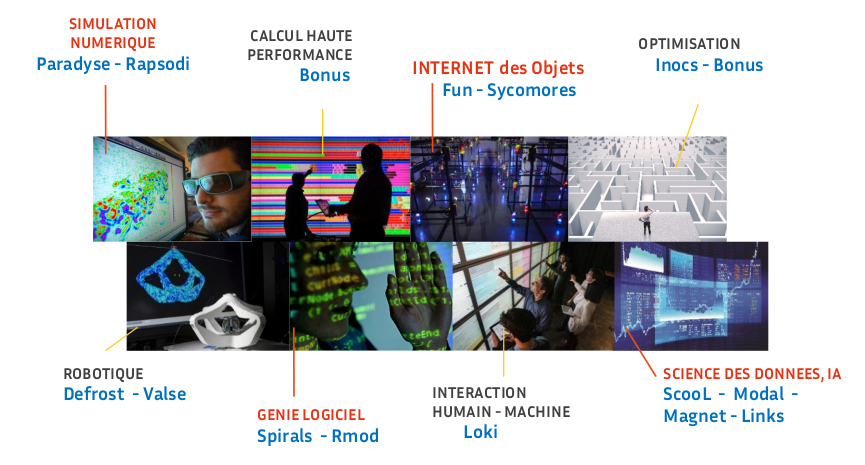
\includegraphics[width=0.55\textwidth]{equipesCentre.png}
	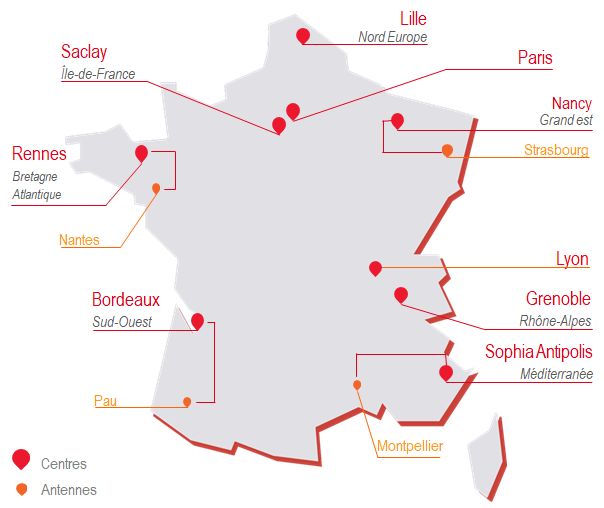
\includegraphics[width=0.4\textwidth]{cartecentres.png}
\end{figure}

\section{Présentation de l'entreprise} \label{PresentationInria}

\subsection{Inria}
Le centre de recherche Inria fondé en 1967 est un établissement publique de recherche se spécialisant dans le domaine des mathématiques et de l'informatique.\\ 
Le centre de Lille Nord Europe fait partie des 9 centres autour de la France et comporte deux complexes: à la Haute Borne et à Euratechnologie. 
Au sein du centre dirigé par Mireille R\'EGNIER operent 15 équipes dont mon équipe d'acceuil: SPIRALS. 

\begin{figure}[h]
	\centering
	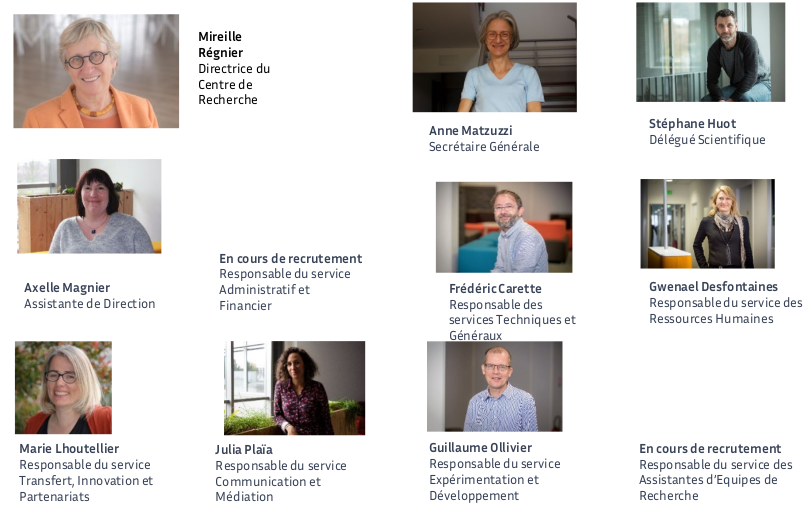
\includegraphics[width=10cm]{direction.png}
	\caption{\'Equipe de direction}
\end{figure}

\subsection{SPIRALS} est une équipe jointe de l'INRIA et de CRISTAL qui se focalise sur les systèmes distribués et l'ingéniérie système. les projets de l'équipe comportent l'étude de solutions autonomes, efficaces et adaptatives pour la récupération et le traitement de données. Dirigée par Lionel Seinturier, l'équipe est actuellement composée de 11 chercheurs permanents, 7 postdocs, 17 doctorants et 7 ingénieurs.

\newpage

\section{Contexte du projet}
\subsection{Introduction aux adBlockers}\label{Intro:adblock}

\paragraph*{Les cookies:}

Le modèle économique du web est centré autour des données utilisateur et de la façon dont elles sont utilisées, majoritairement pour cibler au mieux des publicités qui pourront alors faire un maximum de convertions (nombres d'achats par publicité imprimée sur une page). Evidement pour cibler efficacement un utilisateur il est nécessaire de pouvoir associer un ensemble de données à un utilisateur, historiquement les cookies ont été l'outil le plus répendu pour remplir cette fonction: en incorporant un identifiant unique à chaque utilisateur dans ses requêtes HTML.\\

Malheureusement pour les géants du web, l'idée que quelques entreprises puissent avoir accès à une quantité alarmante de leurs données simplement par leur navigation sur le web ne plait pas vraiment aux utilisateurs. Suite à des campagnes de sensibilisation de plus en plus d'utilisateurs du web se sont retrouvés confrontés à cette réalité et désirent autant que possible limiter l'accès à leurs données de navigation. Pour cela plusieurs compagnies se sont misent à créer des extensions pour navigateurs qui permettent de bloquer les dis ``tracking cookies''. En effet tous les cookies n'ont pas pour but de traquer l'utilisateur, la technologie a été créée pour garder des informations utilisateurs essentielles à la fonctionnalité du site comme rester connecter à son compte utilisateur ou sauvegarder l'état du panier sur les sites de shopping en ligne. Ces cookies dits ``essentiels'' doivent être filtrés pour garder les fonctionnalités du site, une méthode largement utilisée est de bloquer les cookies dits ``tierces'' qui proviennent de domaines différents de celui du site visité étant donné que ceux ci sont bien souvent utilisés uniquement comme tracking cookies et peuvent donc être bloqués sans crainte de nuire aux fonctionnalités du site.

\paragraph*{La publicité sur le web:}

Comme dit précédement, le modèle économique du web consiste à montrer le plus de publicités intéressantes possible à l'utilisateur pour qu'il achète le plus de produits possible. Ce modèle entraîne logiquement un comportement où les sites utilisent chaque pixel d'espace libre de contenu sur leurs sites pour y servir des publicités grâce à un modèle d'enchères où les distributeurs de publicités enchèrissent le plus sur les utilisateurs avec un intérêt probable pour leurs produits.

Les utilisateurs veulent donc se débarasser un maximum des publicités à la fois pour leur confort mais aussi pour protéger les plus vulnérables des pratiques prédatoriales des entreprises. C'est là l'utilité des adBlockers qui scannent les éléments de la page et bloquent ceux qui sont détectés comme étant des publicités.

\paragraph*{Les rêgles de filtrage:}

Pour détecter les élements qui font parties de publicités, les adBlockers utilisent des listes de filtres qui contiennent des caractèristiques d'élements publicitaires rencontrés sur le web. Ces listes sont maintenus régulièrement par la communauté et par des entreprises d'adBlockers pour parer aux nouvelles tentatives de contournement des distributeurs de publicités. Les listes sont de simples fichiers texte dont la syntaxe de base est définie par AdBlockPlus (ABP) \href{https://help.eyeo.com/en/adblockplus/how-to-write-filters#allowlist}{ici} et elle est étendue par uBlockOrigin (uBO) \href{https://github.com/gorhill/uBlock/wiki/Static-filter-syntax#extended-syntax}{ici}. La syntaxe comporte deux grands types de rêgles: 
\begin{itemize}
\item Les \textit{Network Rules}
\item Les \textit{Cosmetic Rules}
\end{itemize}
Le cas le plus simple, les \textit{Network Rules} correspondent à des rêgles qui bloquent les éléments selon l'url dont ils sont importés, ce grâce à une syntaxe similaire à des expressions réguliaires. C'est à dire que la rêgle décrits un modèle d'url qui correspond à un ensemble d'url qui devront être bloquées, par exemple ``http://example.com/ads/banner*.gif'' bloquera les élements venant de la source ``http://example.com/ads/banner420.gif'' (le caractère \textbf{*}\\ correspondant à n'importe quelle suite de caractère) mais pas \\``http://example.fr/ads/ad123.png''.

Plus puissantes, les \textit{Cosmetic Rules} bloquent des élements dont le css correspond à une certaine description, par exemple la rêgle ``\#\#\#ad-boxes'' bloque les élements sur la page qui ont une id css de ``ad-boxes''.

Il est également possible d'écrire des exceptions qui permettent de laisser passer des élements qui seraient bloqués par une rêgle trop générale et qui nuirait aux fonctionnalités du site.

\subsection{Présentation AmIUnique}

\paragraph*{Le Fingerprinting sur le web}

Comme décrit en \ref{Intro:adblock} les cookies ont longtemps été l'outil principal pour suivre les utilisateurs sur le web, mais les efforts des adBlockers et des navigateurs comme Firefox ou Brave ont rendus leurs utilisation plus difficile ou moins efficaces qu'avant, et avec la demande pour les données utilisateur encore grimpante, de nouveaux outils plus avancés sont développés pour continuer à suivre les utilisateurs sur le web. 

Un outil qui remplis cette fonction peut-être mieux encore que les cookies le faisaient auparavant est le \textbf{Browser Fingerprinting} (\cite{fingerprinting}) le principe derrière celui-ci consiste à appliquer une approche inspirée de la \textit{data science} et d'obtenir un maximum de bribes d'information sur l'utilisateur (ou ici plutôt son navigateur) afin de les agréger en un identificateur unique permettant de suivre l'utilisateur grâce à la configuration de son navigateur que les cookies soit acceptés ou non.

\paragraph*{AmIUnique} est un projet d'Inria Lille qui consiste à étudier les caractèristiques du navigateur qui permettent de l'identifier et de faire des statistiques sur les changements de l'identificateur au cours du temps grâce à une extension qui collecte les informations d'identification.

\section{Corps du projet}


\section{Extras}


\newpage

\appendix
\printbibliography

\newpage

\begin{center}
	
	\vspace{2cm}
	\renewcommand{\abstractname}{Résumé}
	\begin{abstract}
	
	Lors de ce stage blablabla

	\end{abstract}
	\textbf{Mots clés: }
	\vspace{\fill}	
	\renewcommand{\abstractname}{Abstract}
	\begin{abstract}
	
	During this internship blablabla

	\end{abstract}
	\textbf{Keywords: }
	\vspace{2cm}

\end{center}





\end{document}